\documentclass[10pt]{beamer}
\usefonttheme{professionalfonts,serif}
\def\newblock{\hskip .11em plus .33em minus .07em}
\usepackage[numbers,sort]{natbib}
\renewcommand{\rmdefault}{psbx}
\usepackage[utf8]{inputenc}
\usepackage[T1]{fontenc}
\usepackage{textcomp}
\usepackage{eulervm}

\usetheme{default}           % tips from David Blei
\useinnertheme{circles}
\useoutertheme{infolines}
\setbeamertemplate{headline}{}
\setbeamertemplate{navigation symbols}{}
\setbeamerfont{itemize/enumerate subbody}{size=\normalsize}
\setbeamerfont{itemize/enumerate subsubbody}{size=\normalsize}
\usecolortheme{seahorse}
\setbeamersize{text margin left=2mm,text margin right=2mm}

\graphicspath{{../../figures/}}

\definecolor{mypine}{rgb}{0.05,0.45,0.05}
\definecolor{mycyan}{rgb}{0.0,0.9,0.9}
\newcommand{\Red}{\textcolor{red}}
\newcommand{\Blue}{\textcolor{blue}}
\newcommand{\Green}{\textcolor{mypine}}
\newcommand{\PineGreen}{\textcolor{mypine}}
\newcommand{\Magenta}{\textcolor{magenta}}
\newcommand{\Cyan}{\textcolor{mycyan}}

\newcommand{\N}{\mathcal{N}}
\newcommand{\R}{\mathbb{R}}
\newcommand{\T}{{\scriptsize^{\top}}}
\newcommand{\D}{\mathcal{D}}
\newcommand{\F}{\mathcal{F}}
\newcommand{\E}{\mathbb{E}}
\newcommand{\V}{\mathbb{V}}
\newcommand{\M}{\mathcal{M}}
\newcommand{\KL}{\mathcal{KL}}
\newcommand{\cut}[1]{}
\newcommand{\trace}{\operatorname{trace}}

\newcommand{\bmu}{{\boldsymbol{\mu}}}
\newcommand{\btheta}{\boldsymbol{\theta}}
\newcommand{\bepsilon}{\boldsymbol{\epsilon}}
\newcommand{\balpha}{\boldsymbol{\alpha}}
\newcommand{\bbeta}{\boldsymbol{\beta}}
\newcommand{\bphi}{\boldsymbol{\phi}}
\newcommand{\bPhi}{\boldsymbol{\Phi}}
\newcommand{\bSigma}{\boldsymbol{\Sigma}}
\newcommand{\bpi}{\boldsymbol{\pi}}
\newcommand{\blambda}{\boldsymbol{\lambda}}

\newcommand{\argmax}{\operatorname{argmax}}
\newcommand{\argmin}{\operatorname{argmin}}
\newcommand{\ci}{{\bot\negthickspace\negthickspace\bot}} % conditional indep.
\newcommand{\neigh}{\operatorname{ne}}
\newcommand{\vectr}[2]{  \left[ \!\!\begin{array}{c} #1 \\
      #2 \end{array} \!\!\right]}
\newcommand{\deff}{\stackrel{\mathrm{def}}{=}}
\newcommand{\deldel}[2]{\frac{\partial #1}{\partial #2}}

\newcommand{\maketilde}{\raisebox{0.4ex}{\tiny $\sim$}}
\newcommand{\bfa}{\mathbf a}
\newcommand{\bfb}{\mathbf b}
\newcommand{\bfe}{\mathbf e}
\newcommand{\bff}{\mathbf f}
\newcommand{\bfk}{\mathbf k}
\newcommand{\bfm}{\mathbf m}
\newcommand{\bfn}{\mathbf n}
\newcommand{\bfp}{\mathbf{p}}
\newcommand{\bfs}{\mathbf s}
\newcommand{\bfu}{\mathbf u}
\newcommand{\bfx}{\mathbf x}
\newcommand{\bfy}{\mathbf y}
\newcommand{\bft}{\mathbf t}
\newcommand{\bfv}{\mathbf v}
\newcommand{\bfw}{\mathbf w}
\newcommand{\bfA}{\mathbf A}
\newcommand{\bfI}{\mathbf I}
\newcommand{\bfK}{\mathbf K}


\title{Linear in the parameters regression}
\author{Carl Edward Rasmussen}
\date{October 9th, 2023}

\begin{document}

\begin{frame}
\titlepage
\end{frame}

\begin{frame}
\frametitle{How do we fit this dataset?}

\centerline{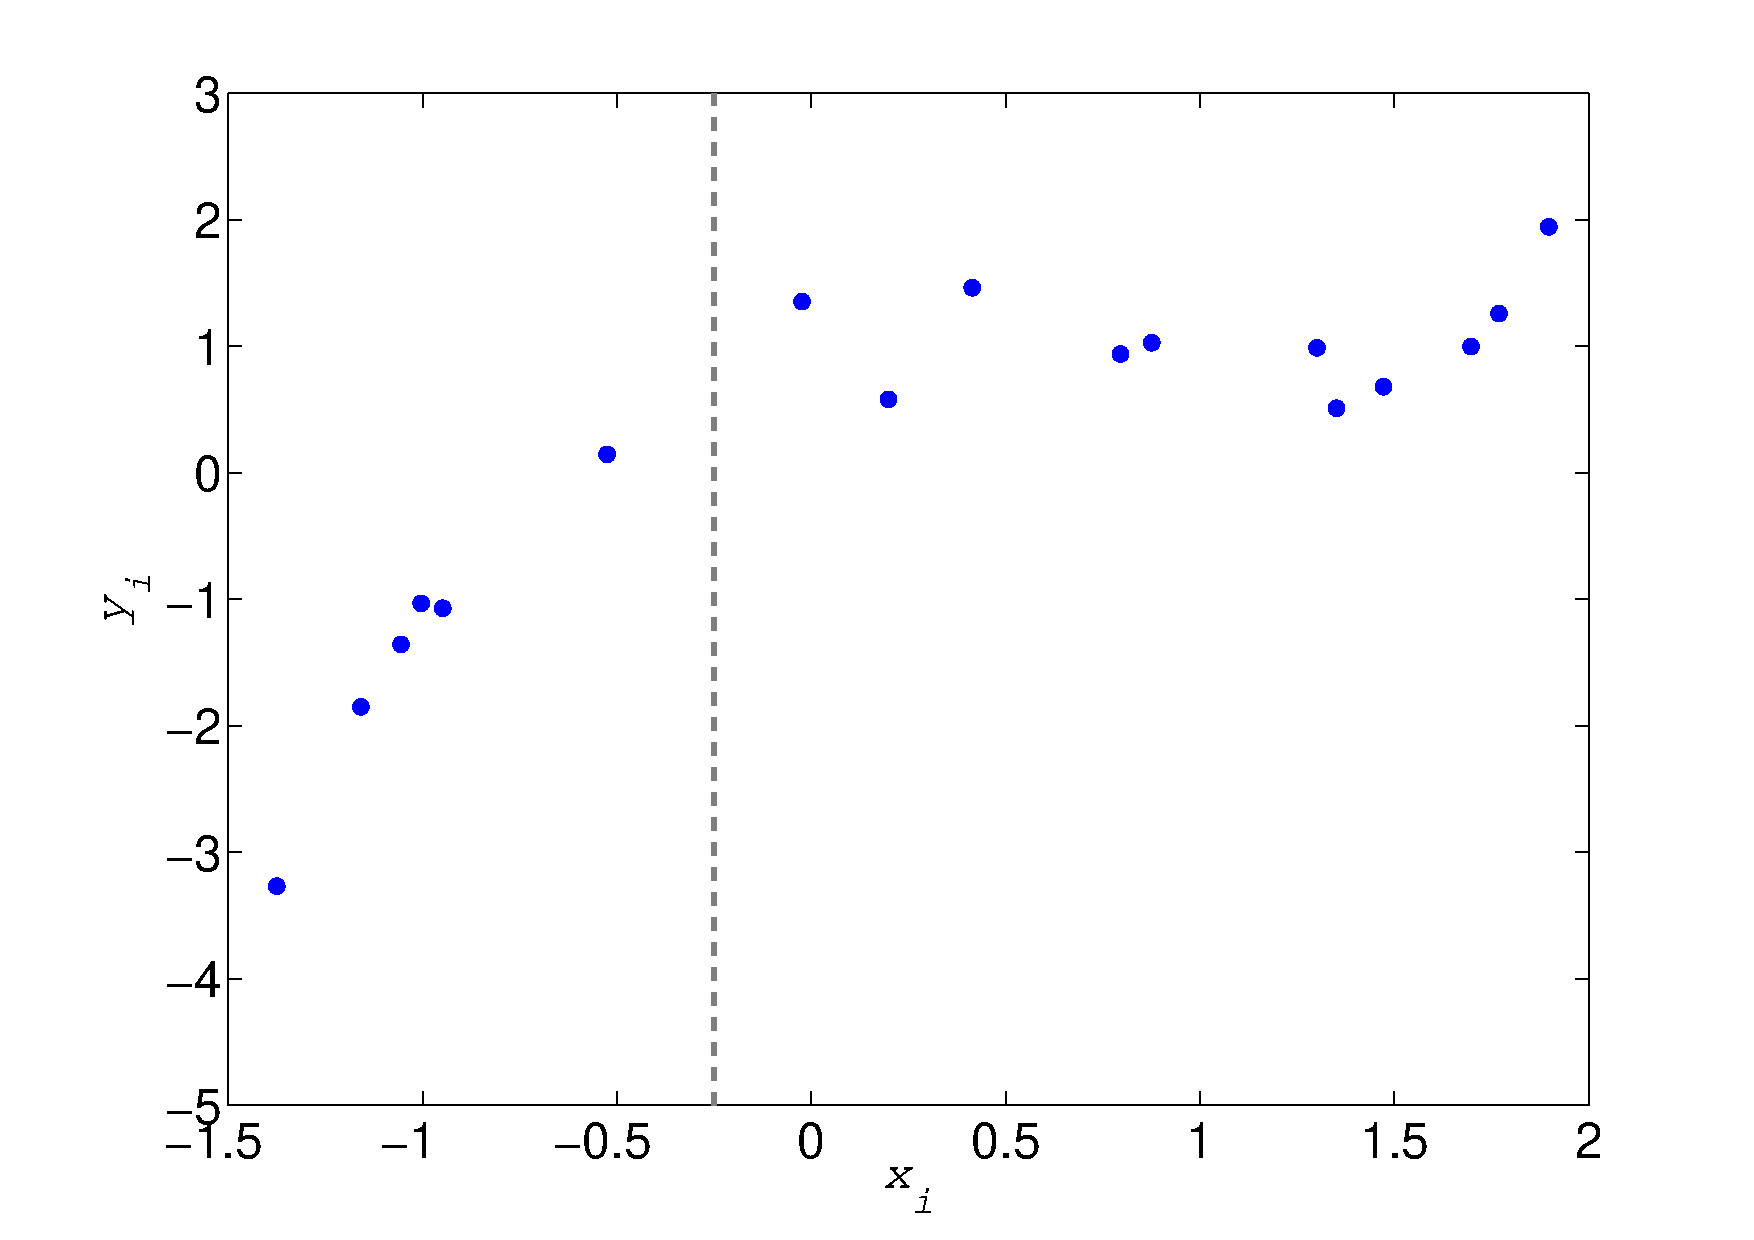
\includegraphics[width=0.5\textwidth]{toy_data.pdf}}

\vfill

\begin{itemize}
\item Dataset ${\cal D}=\{x_i,y_i\}_{i=1}^N$ of $N$ pairs of inputs 
$x_i$ and  targets $y_i$.\\ This data can for example be
measurements in an experiment.
\item Goal: predict target $y_*$ associated to any arbitrary input 
$x_*$.\\ This is known a as a \Blue{regression} task in machine learning.
\item Note: Here the inputs are scalars, we have a single \Blue{input feature}.\\ 
Inputs to regression tasks are often vectors of multiple input features.
\end{itemize}
\end{frame}

%%%%%%%%%%%%%%%%%%%%%%%%%%%%%%%%%%%%%%%%%%%%%%%%%%%%%%%%%%%%%%%%%%%%%%
\begin{frame}
\frametitle{Model of the data}

\centerline{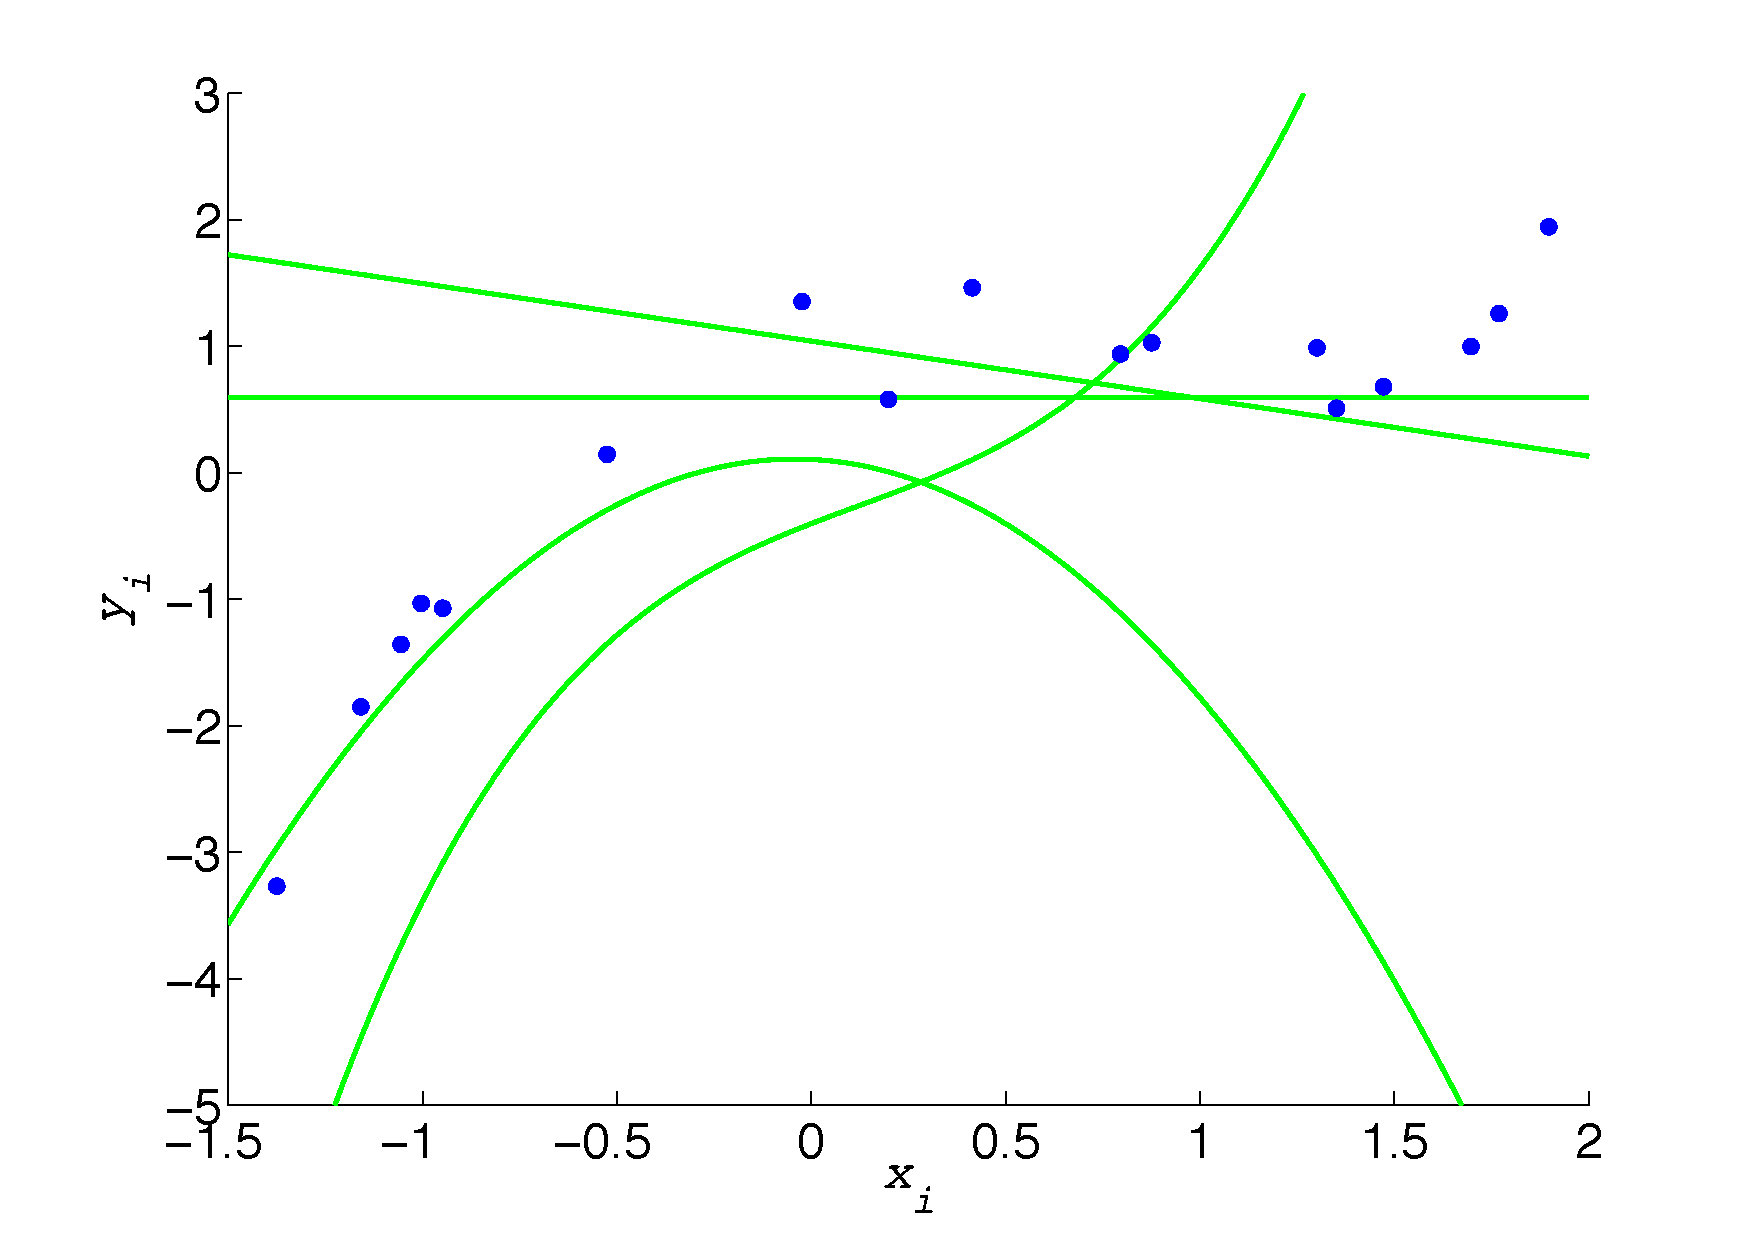
\includegraphics[width=0.5\textwidth]{few_random_polynomials.pdf}}

\vfill

\begin{itemize}
\item In order to predict at a new $x_*$ we need to postulate a model of the data.\\
We will estimate $y_*$ with $f(x_*)$.
\item But what is $f(x)$? Example: a polynomial
%
\[
f_{\bm w}(x)\;=\; w_0 + w_1\,x + w_2\,x^2 + w_3\,x^3 + \ldots + w_M\,x^M
\]
%
The $w_j$ are the weights of the polynomial, the \Blue{parameters} of the model.
\end{itemize}


\end{frame}
%%%%%%%%%%%%%%%%%%%%%%%%%%%%%%%%%%%%%%%%%%%%%%%%%%%%%%%%%%%%%%%%%%%%%%
\begin{frame}
\frametitle{Model of the data. Example: polynomials of degree \sf{M}}

\centerline{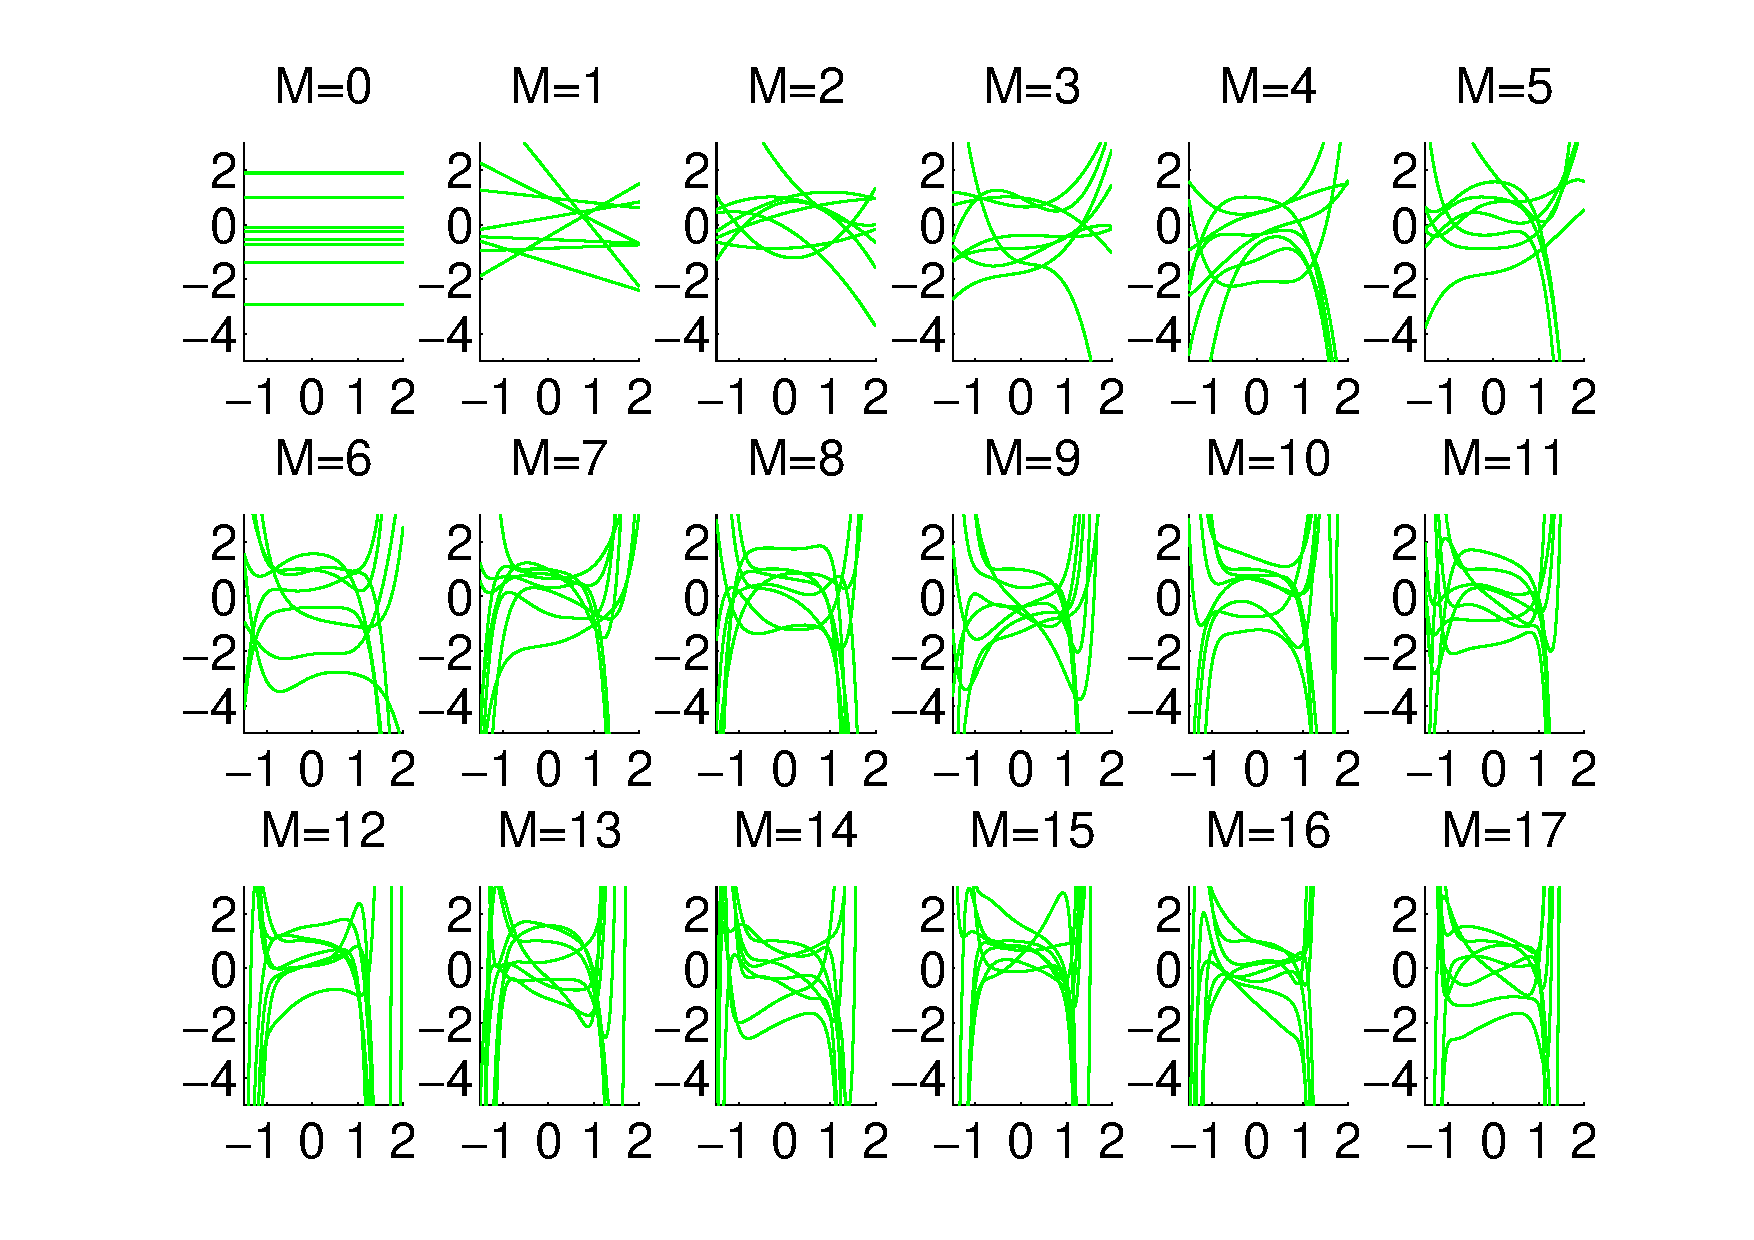
\includegraphics[width=\textwidth]{random_polynomials.pdf}}

\end{frame}
%%%%%%%%%%%%%%%%%%%%%%%%%%%%%%%%%%%%%%%%%%%%%%%%%%%%%%%%%%%%%%%%%%%%%%
\begin{frame}
\frametitle{Model structure and model parameters}

\centerline{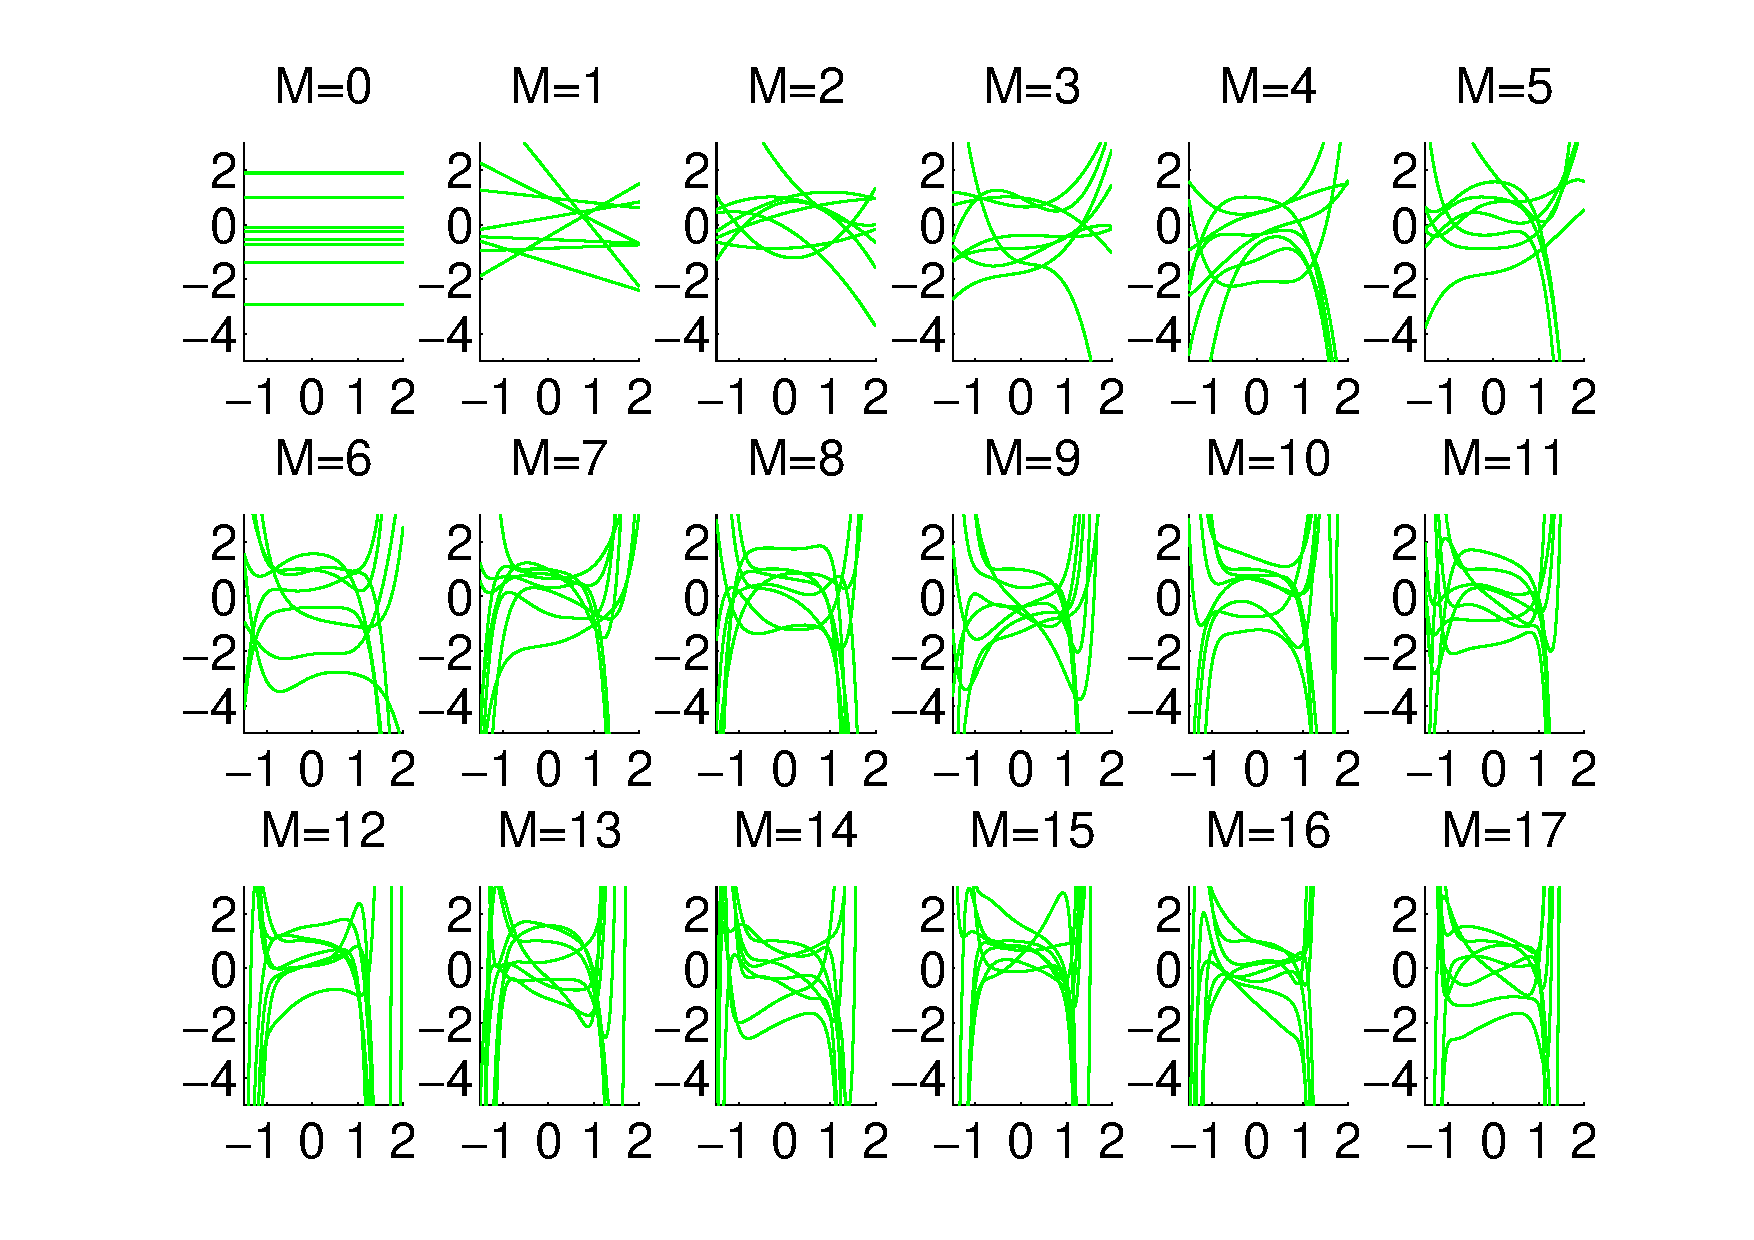
\includegraphics[width=0.5\textwidth]{random_polynomials.pdf}}

\begin{itemize}
\item Should we choose a polynomial? \hfill\Blue{model structure}
\item What degree should we choose for the polynomial? \hfill\Blue{model structure}
\item For a given degree, how do we choose the weights? \hfill\Blue{model parameters}
\item For now, let find the single ``best'' polynomial: degree and weights.
\end{itemize}


\end{frame}
%%%%%%%%%%%%%%%%%%%%%%%%%%%%%%%%%%%%%%%%%%%%%%%%%%%%%%%%%%%%%%%%%%%%%%
\begin{frame}
\frametitle{Fitting model parameters: the least squares approach}

\centerline{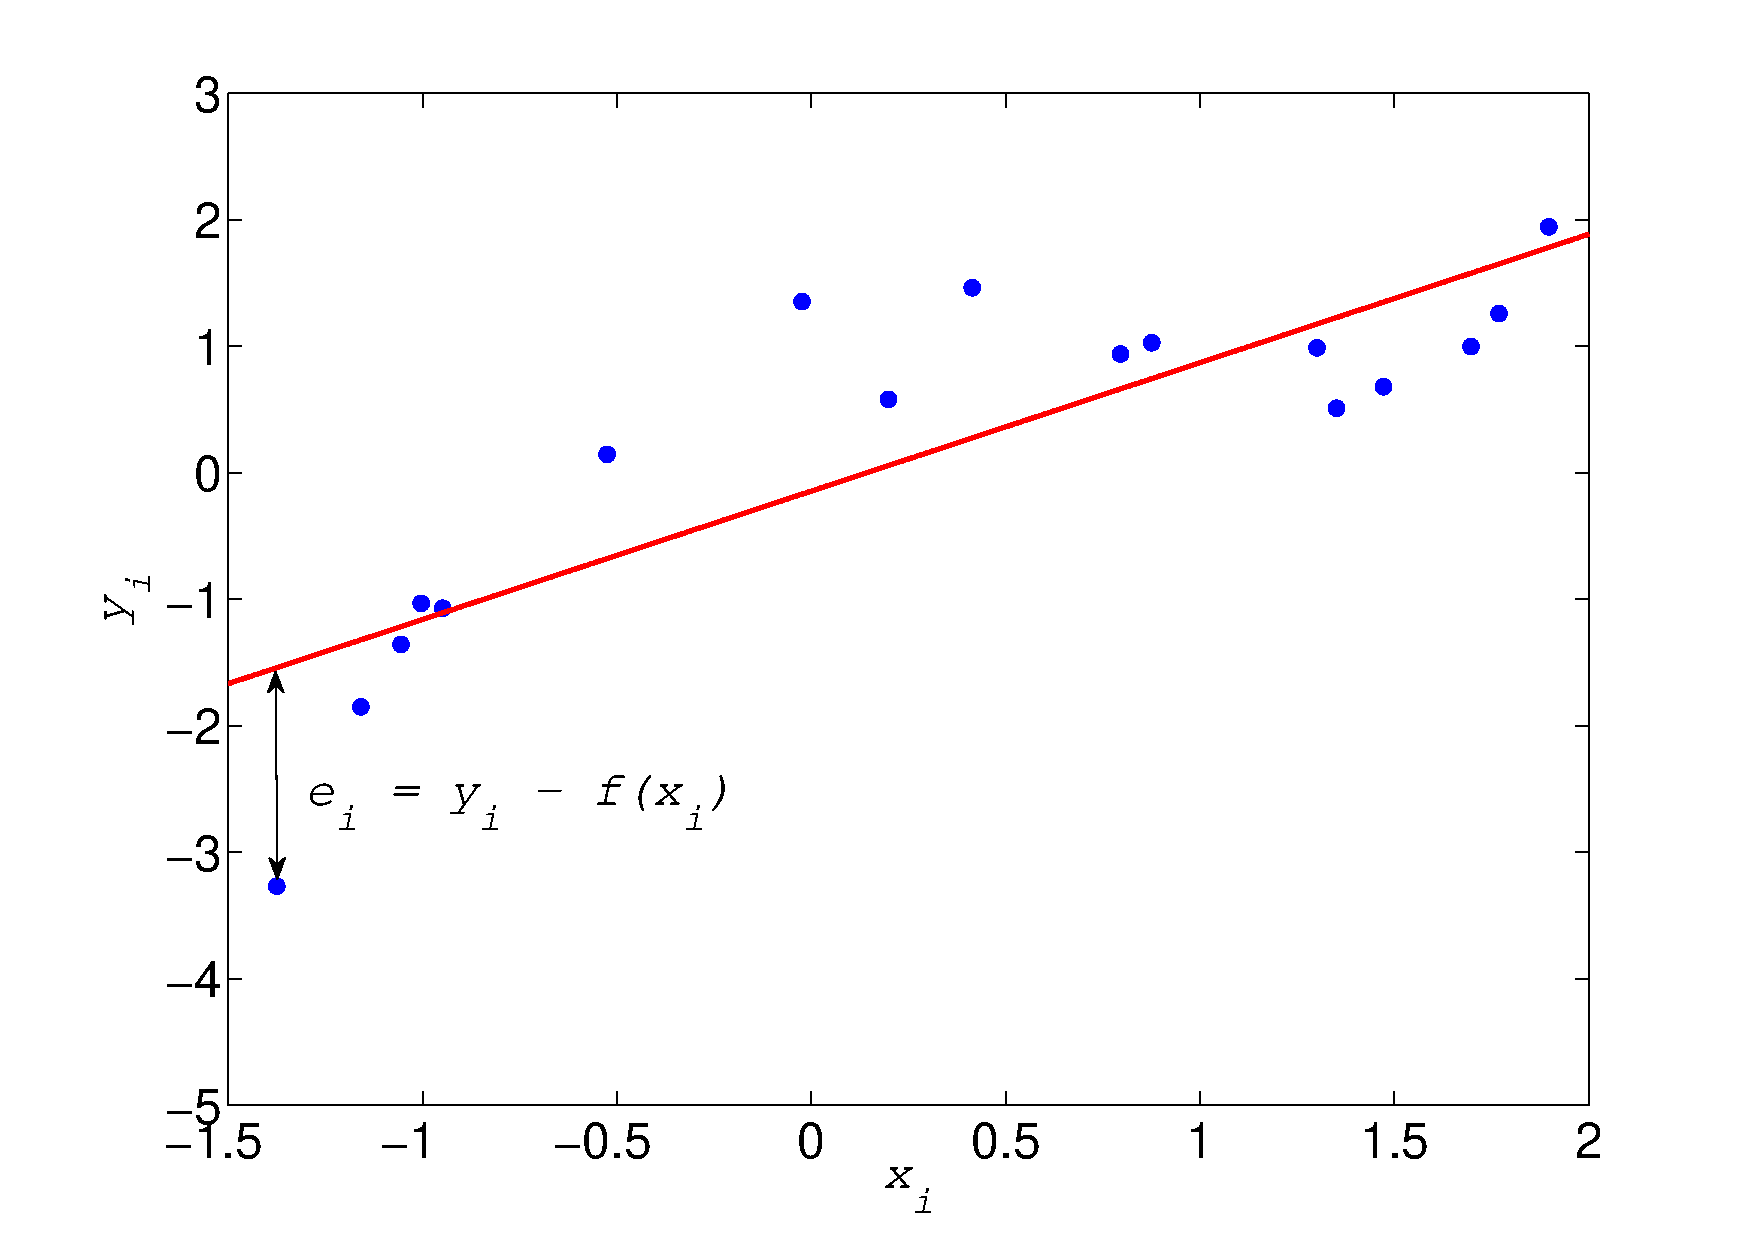
\includegraphics[width=0.5\textwidth]{toy_data_example_fit.pdf}}

\begin{itemize}
\item Idea: measure the quality of the fit to the training data.
\item For each training point, measure the squared error $e_i^2=(y_i-f(x_i))^2$.
\item Find the parameters that minimise the sum of squared errors:
%
\[
E(\bfw)\;=\;\sum_{i=1}^N e_i^2
\]
%
$f_{\bm w}(x)$ is a function of the parameter vector 
$\bfw=[w_0, w_1, \ldots, w_M]\T$.
\end{itemize}


\end{frame}
%%%%%%%%%%%%%%%%%%%%%%%%%%%%%%%%%%%%%%%%%%%%%%%%%%%%%%%%%%%%%%%%%%%%%%
\begin{frame}
\frametitle{Least squares in detail. (1) Notation}

Some notation: training targets $\bfy$, predictions $\bff$ and errors $\bfe$.
\begin{itemize}
\item $\bfy=[y_1,\ldots,y_N]^\top$ is a vector that stacks the $N$ training targets.
\item $\bff=[f_{\bm w}(x_1), \ldots, f_{\bm w}(x_N)]^\top$  stacks
  $f_{\bm w}(x)$ evaluated at 
the $N$ training inputs.
\item $\bfe=\bfy-\bff$ is the vector of training prediction errors.
\end{itemize}
The sum of squared errors is therefore given by
%
\[
E(\bfw)\;=\; \|\bfe\|^2\;=\;\bfe^\top\bfe\;=\;(\bfy-\bff)^\top(\bfy-\bff)
\]
%
More notation: weights $\bfw$, basis functions $\phi_j(x)$ and matrix $\bPhi$.
\begin{itemize}
\item $\bfw=[w_0, w_1, \ldots, w_M]^\top$ stacks the $M+1$ model weights.
\item $\Red{\phi_j(x)}=x^j$ is a \Red{basis function} of our \Blue{linear in the parameters} 
model.
%
\[
f_{\bm w}(x)\; =\; \Blue{w_0}\,\Red{1} + \Blue{w_1}\,\Red{x} + \Blue{w_2}\,\Red{x^2} + 
\ldots + \Blue{w_M}\,\Red{x^M}\; =\; \sum_{j=0}^M \Blue{w_j}\,\Red{\phi_j(x)}
\]
%
\item $\bPhi_{ij}=\phi_j(x_i)$ allows us to write $\bff=\bPhi\,\bfw$.
\end{itemize}

\end{frame}
%%%%%%%%%%%%%%%%%%%%%%%%%%%%%%%%%%%%%%%%%%%%%%%%%%%%%%%%%%%%%%%%%%%%%%
\begin{frame}
\frametitle{Least squares in detail. (2) Solution}

\Blue{A Gradient View.} The sum of squared errors is a convex function of $\bfw$:
%
\[
E(\bfw)\;=\;(\bfy-\bff)^\top(\bfy-\bff)\;=\;(\bfy-\bPhi\,\bfw)^\top(\bfy-\bPhi\,\bfw)
\]
%
The gradient with respect to the weights is:
%
\[
\deldel{E(\bfw)}{\bfw}\;=\;-2\,\bPhi^\top(\bfy-\bPhi\,\bfw)
\;=\;2\bPhi^\top\,\bPhi\,\bfw-2\,\bPhi^\top\,\bfy.
\]
%
The weight vector $\hat\bfw$ that sets the gradient to zero minimises $E(\bfw)$:
\[
\boxed{
%
\hat\bfw\;=\;(\bPhi^\top\,\bPhi)^{-1}\,\bPhi^\top\,\bfy
%
}       
\]
\Blue{A Geometrical View.} This is the matrix form of the \Blue{Normal equations}. 
\begin{itemize}
\item The vector of training targets $\bfy$ lives in an $N$-dimensional vector space.
\item The vector of training predictions $\bff$ lives in the same space, but it is constrained
to being generated by the $M+1$ columns of matrix $\bPhi$.
\item The error vector $\bfe$ is minimal if it is orthogonal to all columns of $\bPhi$:
%
\[
\bPhi^\top\,\bfe\;=\;\mathbf{0}\; \iff\; \bPhi^\top\,(\bfy-\bPhi\,\bfw)\;=\;\mathbf{0}
\]
%
\end{itemize}


\end{frame}
%%%%%%%%%%%%%%%%%%%%%%%%%%%%%%%%%%%%%%%%%%%%%%%%%%%%%%%%%%%%%%%%%%%%%%
\begin{frame}
\frametitle{Least squares fit for polynomials of degree 0 to 17}

\centerline{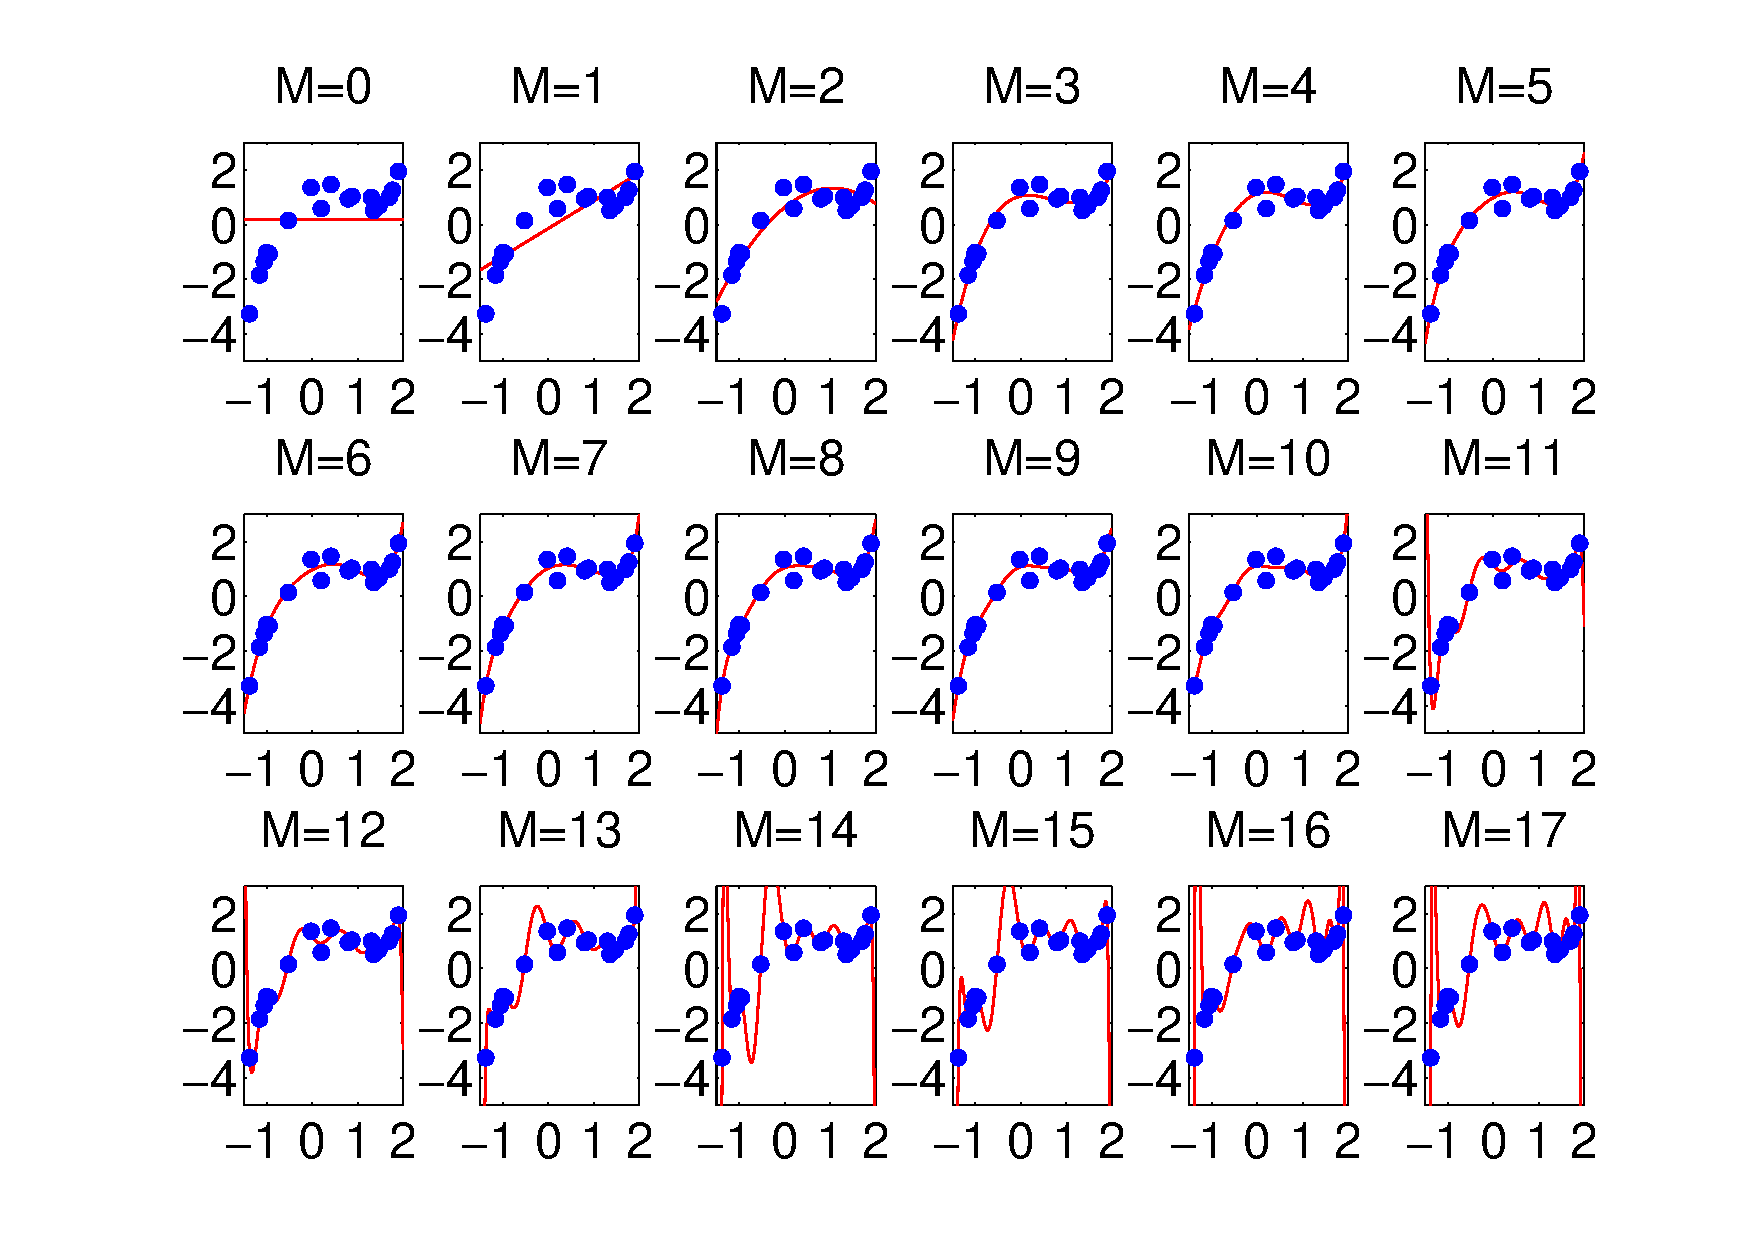
\includegraphics[width=\textwidth]{fitted_polynomials.pdf}}

\end{frame}
%%%%%%%%%%%%%%%%%%%%%%%%%%%%%%%%%%%%%%%%%%%%%%%%%%%%%%%%%%%%%%%%%%%%%%
\begin{frame}
\frametitle{Have we solved the problem?}

\centerline{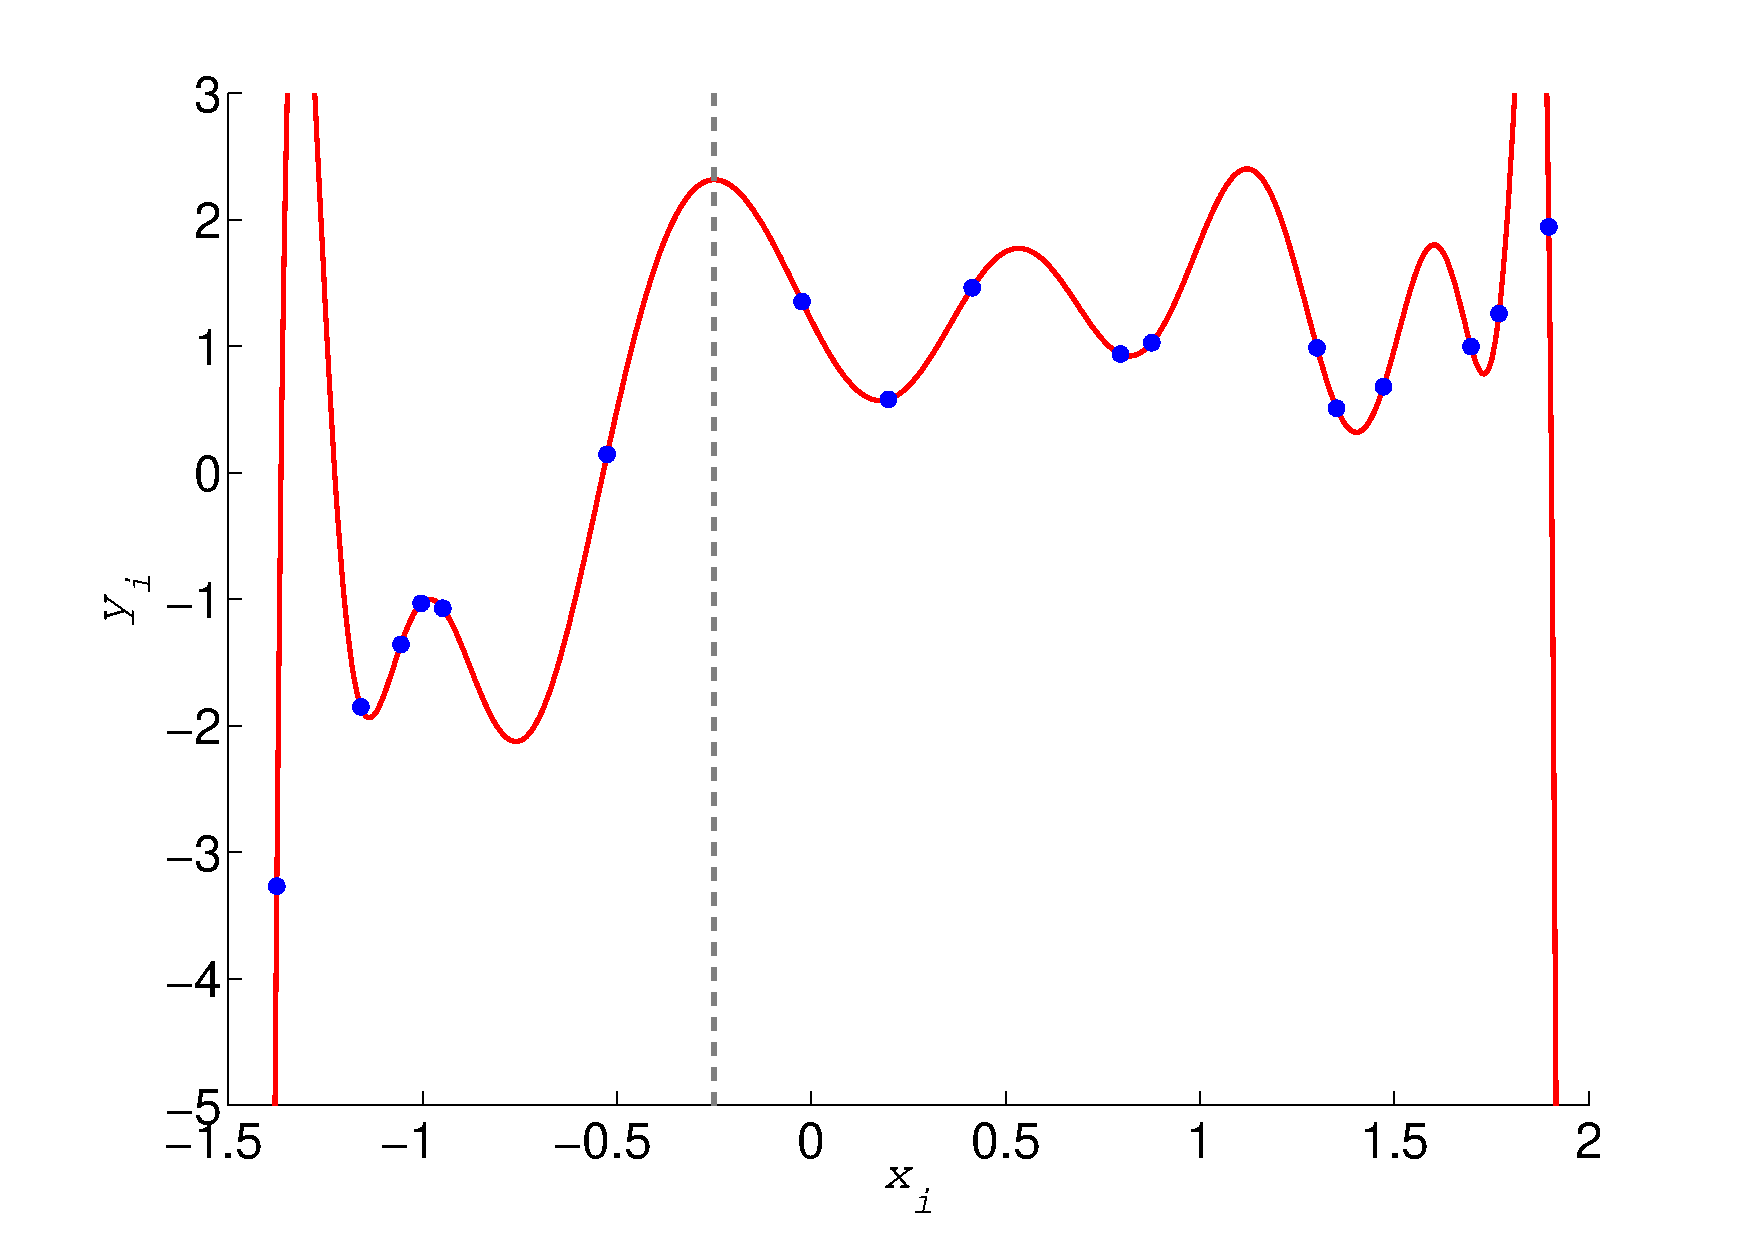
\includegraphics[width=0.7\textwidth]{toy_data_polynomial_overfit.pdf}}

\begin{itemize}
\item Ok, so have we solved the problem?
\item What do we think $y_*$ is for $x_*=-0.25$? And for $x_*=2$?
\item If $M$ is large enough, we can find a model that fits the data 
\end{itemize}


\end{frame}
%%%%%%%%%%%%%%%%%%%%%%%%%%%%%%%%%%%%%%%%%%%%%%%%%%%%%%%%%%%%%%%%%%%%%%
\begin{frame}
\frametitle{Overfitting}

\centerline{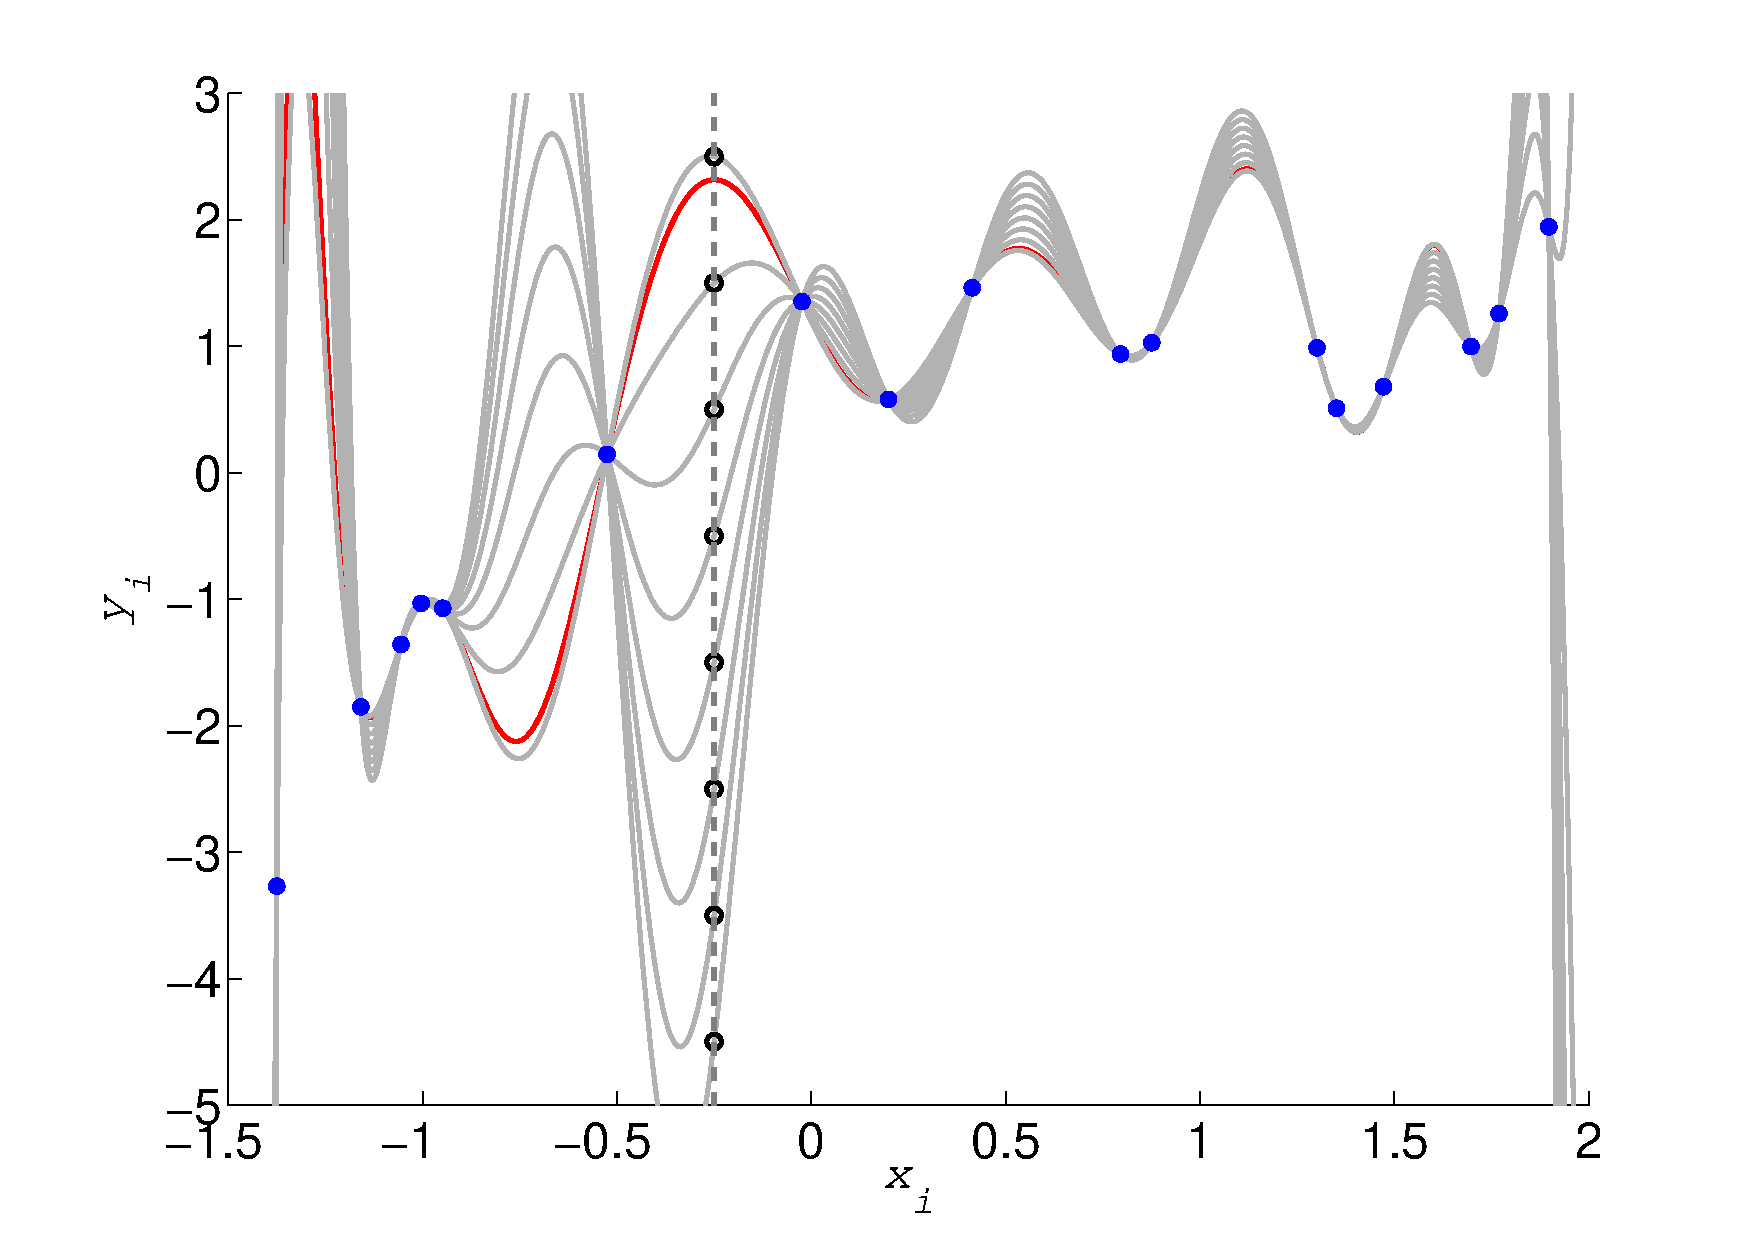
\includegraphics[width=0.7\textwidth]{toy_data_polynomial_choose_your_target.pdf}}

\begin{itemize}
\item All the models in the figure are polynomials of degree 17 (18 weights).
\item All perfectly fit the 17 training points, plus any desired $y_*$ at $x_*=-0.25$.
\item We have not solved the problem. Key missing ingredient: \Blue{\bf assumptions!}
\end{itemize}
\end{frame}

\begin{frame}
\frametitle{Some open questions}

\begin{itemize}
\item Do we think that all models are equally probable... \Red{before} we see any data?\\[1ex]
\hfill \Blue{What does the probability of a model even mean?}\\[4ex]
\item Do we need to choose a single ``best'' model or can we consider several?\\[1ex] 
\hfill \Blue{We need a framework to answer such questions.}\\[4ex]
\item Perhaps our training targets are contaminated with noise. What to do?\\[1ex]
\hfill \Blue{This question is a bit easier, we will start here.}
\end{itemize}
\end{frame}

\end{document}
